% Nome do capítulo
\chapter{Desenvolvimento}
% Label para referenciar
\label{ch:desenvolvimento}

% Diminuir espaçamento entre título e texto
\vspace{-1.9cm}
O desenvolvimento desse trabalho se deu em duas etapas: montagem do \textit{Hardware} e implementação do \textit{Software}. Cada uma dessas etapas será descrita nas próximas seções.

\section{\textit{Hardware}} % (fold)
\label{sec:met_hardware}

Nesta etapa foi utilizada uma luva de material diferente a fim de corrigir o problema da fixação dos sensores nos dedos e para comparação dos protótipos foi elaborado um novo circuito utilizando um \textit{shield} de prototipagem para \textit{Arduino} com conectores que permitem que os sensores de flexão sejam ligados a qualquer um dos \textit{shields}.

\subsection{Luva} % (fold)
\label{sub:luva}
Na luva original de \citeonline{roversi}, os sensores de flexão desviavam muito de suas posições ideais quando se dobrava os dedos, o que causava leituras incorretas, principalmente no polegar e no dedo mínimo. Isso ocorria pelo fato da luva não ficar justa com a mão do usuário e do tecido da luva deformar com facilidade. Devido a isso, foi necessária a escolha de uma nova luva que se prendesse mais à mão do usuário e  com um tecido que não deformasse, permitindo uma melhor fixação dos sensores.

A luva escolhida, mostrada na Figura \ref{fig:luva_neoprene}, é feita de neoprene, um tipo de borracha sintética muito utilizada para equipamentos de mergulho, sendo flexível e resistente. Este material foi escolhido pela sua elasticidade, possibilitando se adaptar a diferentes tamanhos de mãos e garantindo que os sensores de flexão não se desloquem durante o uso do dispositivo.

\begin{figure}[H]
  \setlength{\abovecaptionskip}{0pt}
  \setlength{\belowcaptionskip}{0pt}
  \caption[Luva de neoprene utilizada]{Luva de neoprene utilizada}
  \centering
  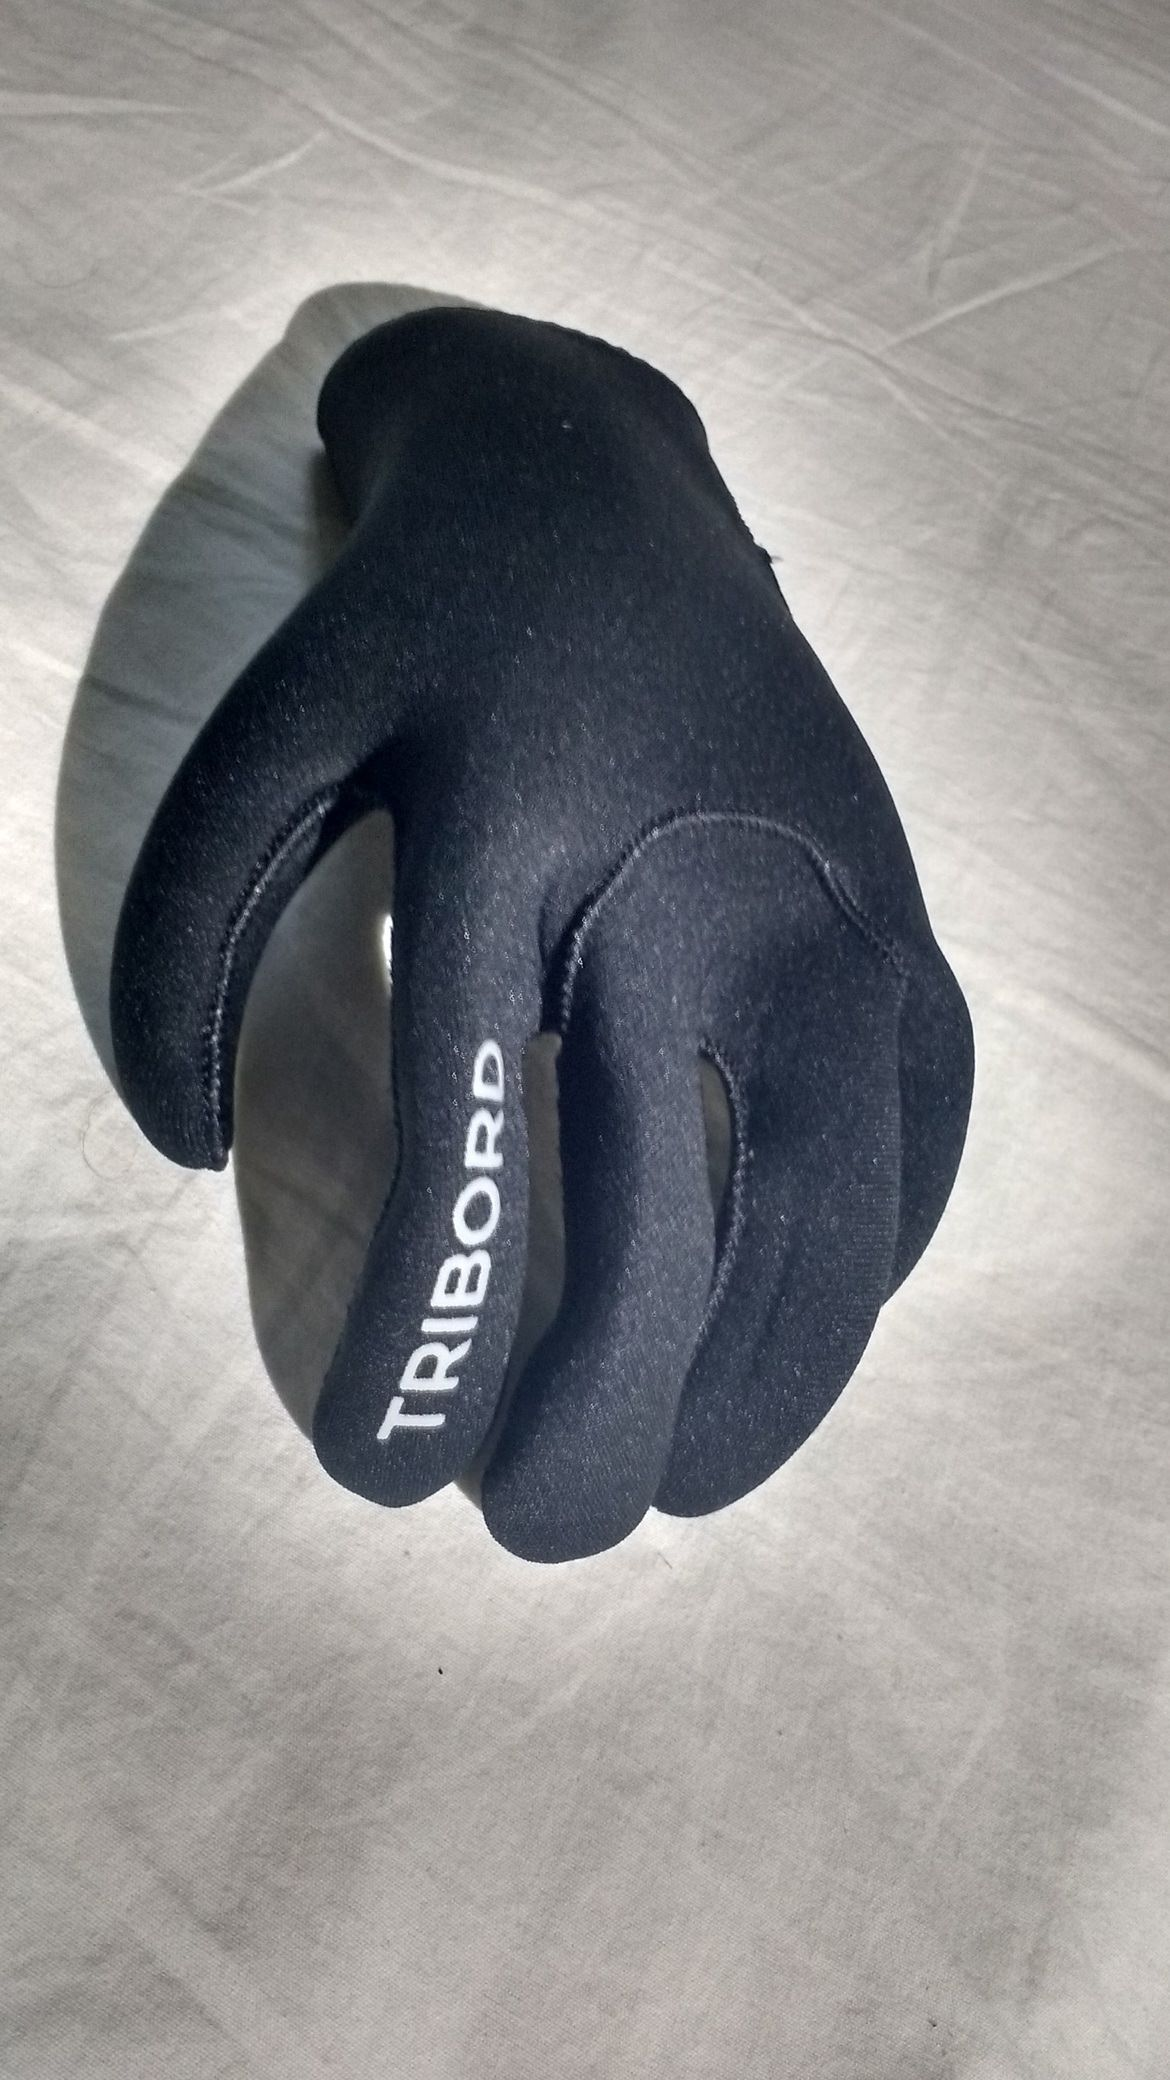
\includegraphics[trim=0 400 100 200,clip,width=.4\textwidth,angle=90]{imagem/luvaneoprene}
  \captionsetup{justification=centering}
  \captionfont{\small{\textbf{\\Fonte: Elaborado pelo Autor}}}
  \label{fig:luva_neoprene}
\end{figure}

% subsubsection luva (end)

\subsection{Sensores de Flexão} % (fold)
\label{sub:sensores_de_flexao}
Os sensores de flexão utilizados foram os mesmos do protótipo de \citeonline{roversi}, detalhados na Seção \ref{sec:sens}. Foram utilizados 14 sensores no total, sendo 5 para captar as dobras das articulações \ac{IFD} e \ac{IFP}, 5 para as articulações \ac{MCF} e 4 para detectar os movimentos de adução e abdução dos dedos. As articulações estão representadas na Figura \ref{fig:art}. Os sensores foram posicionados sobre a mão de forma que fiquem aproximadamente sobre os ossos, para garantir que eles se dobrem de maneira mais semelhante possível ao movimento que o usuário realiza.

A fixação dos sensores na luva foi feita com linha de costura na 1ª, 2ª e 3ª falange de cada dedo, para impedir que o sensor se movimente lateralmente, mas ainda consiga seguir a dobra do dedo do usuário. Para impedir que os sensores deslizem para frente ou para trás, eles também foram fixados com costura em suas bases. A Figura \ref{fig:luva_frente} apresenta os sensores na luva. Os sensores de adução e abdução foram posicionados conforme a Figura \ref{fig:novaluva} e fixados com linha de costura em suas duas extremidades. O ponto de fixação foi entre as articulações \ac{MCF} e \ac{IFP}, para que eles não dificultem os movimentos de flexão.

Ainda foi colocada uma outra luva de \textit{lycra} por cima da luva de neoprene (Figura \ref{fig:luva_lycra}) para auxiliar os sensores a dobrarem quando as articulações \ac{IFD} fossem movimentadas.

\begin{figure}[H]
  \setlength{\abovecaptionskip}{0pt}
  \setlength{\belowcaptionskip}{0pt}
  \caption[Montagem final da Luva]{Montagem final da Luva}
  \centering
  \subfloat[Sensores de flexão na luva]{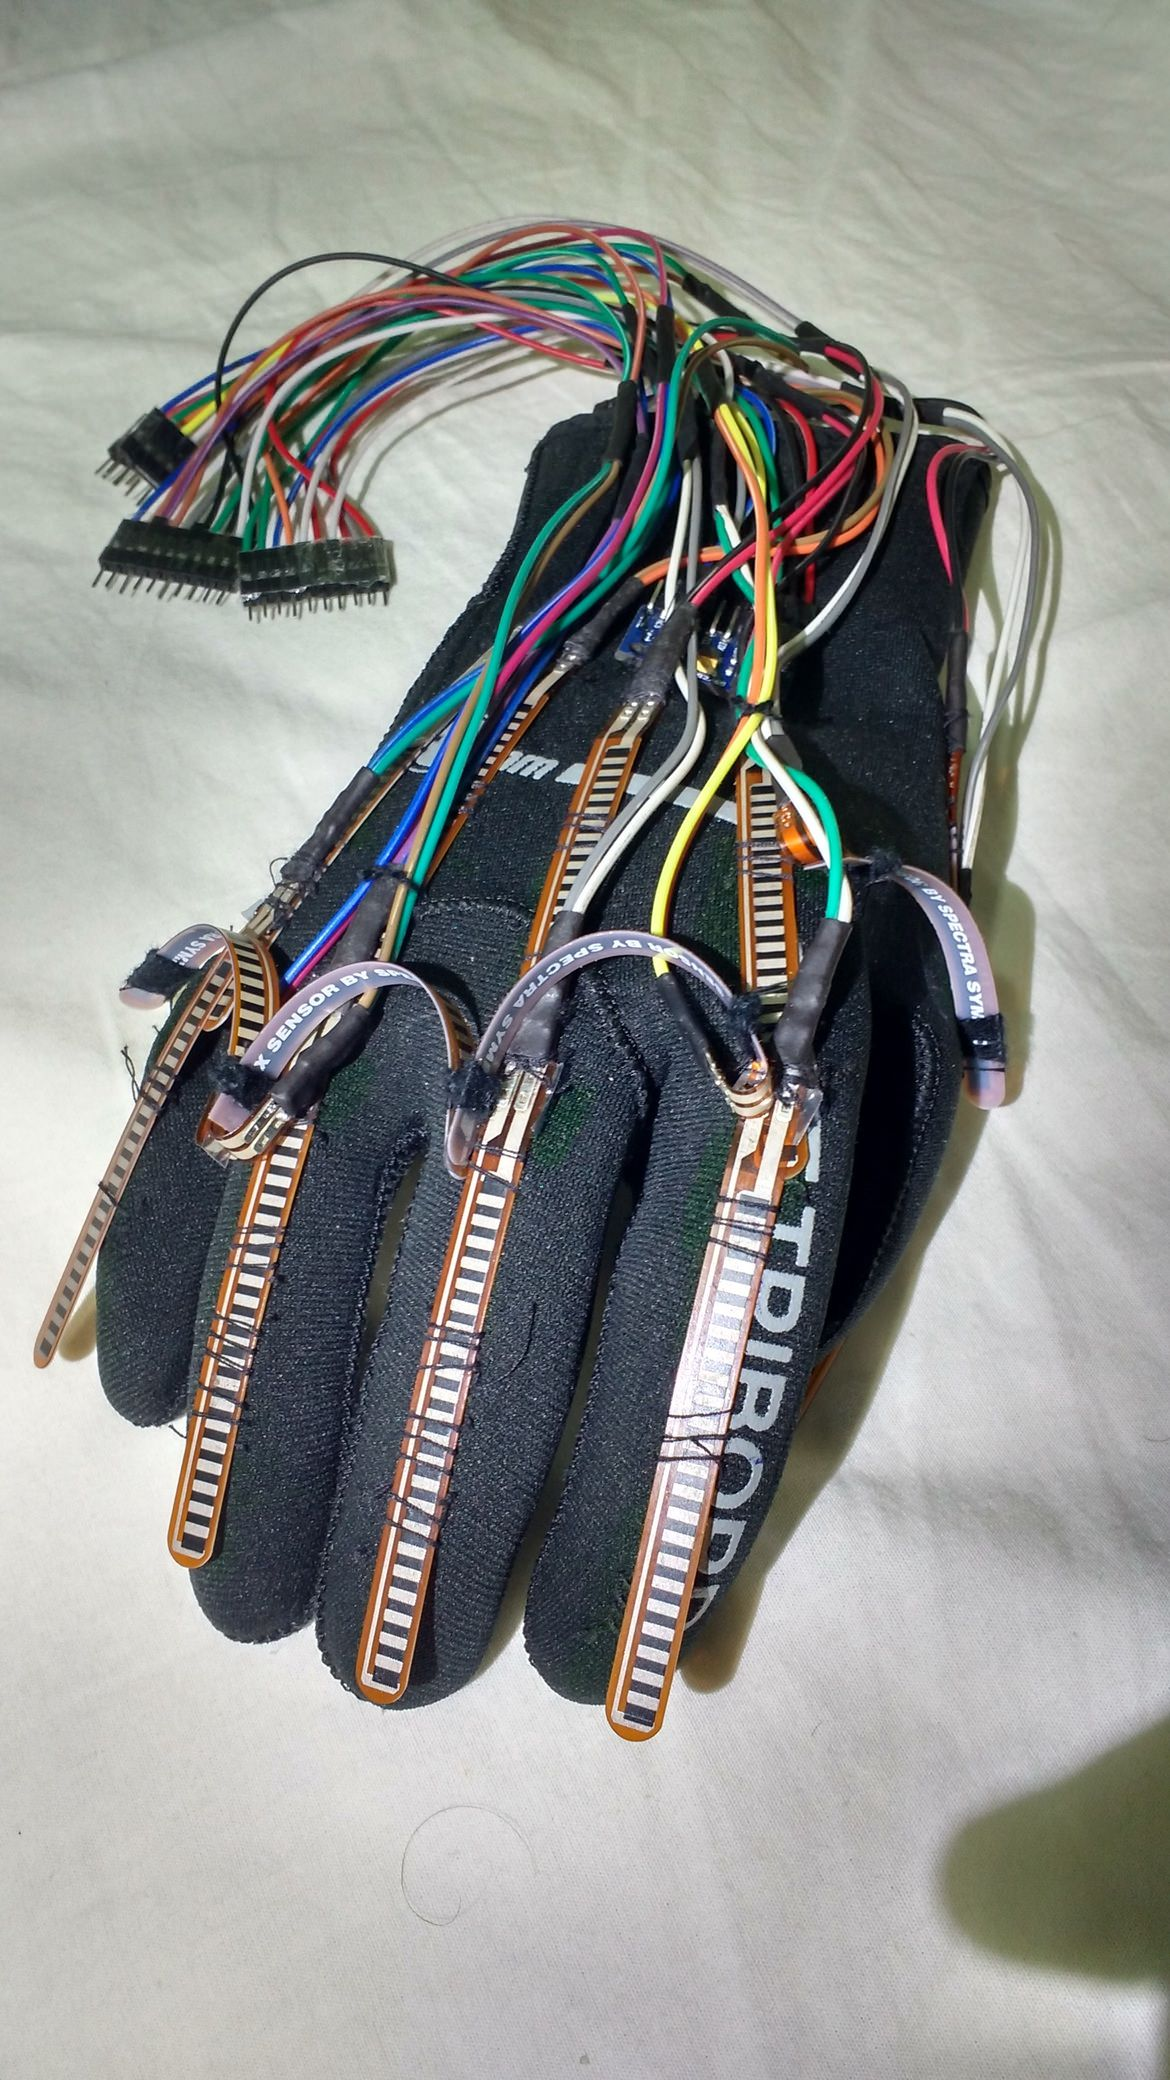
\includegraphics[trim=0 300 100 200,clip,width=.4\textwidth]{imagem/LuvaFrente}\label{fig:luva_frente}}
  \qquad
  \subfloat[Luva de \textit{lycra} cobrindo sensores]{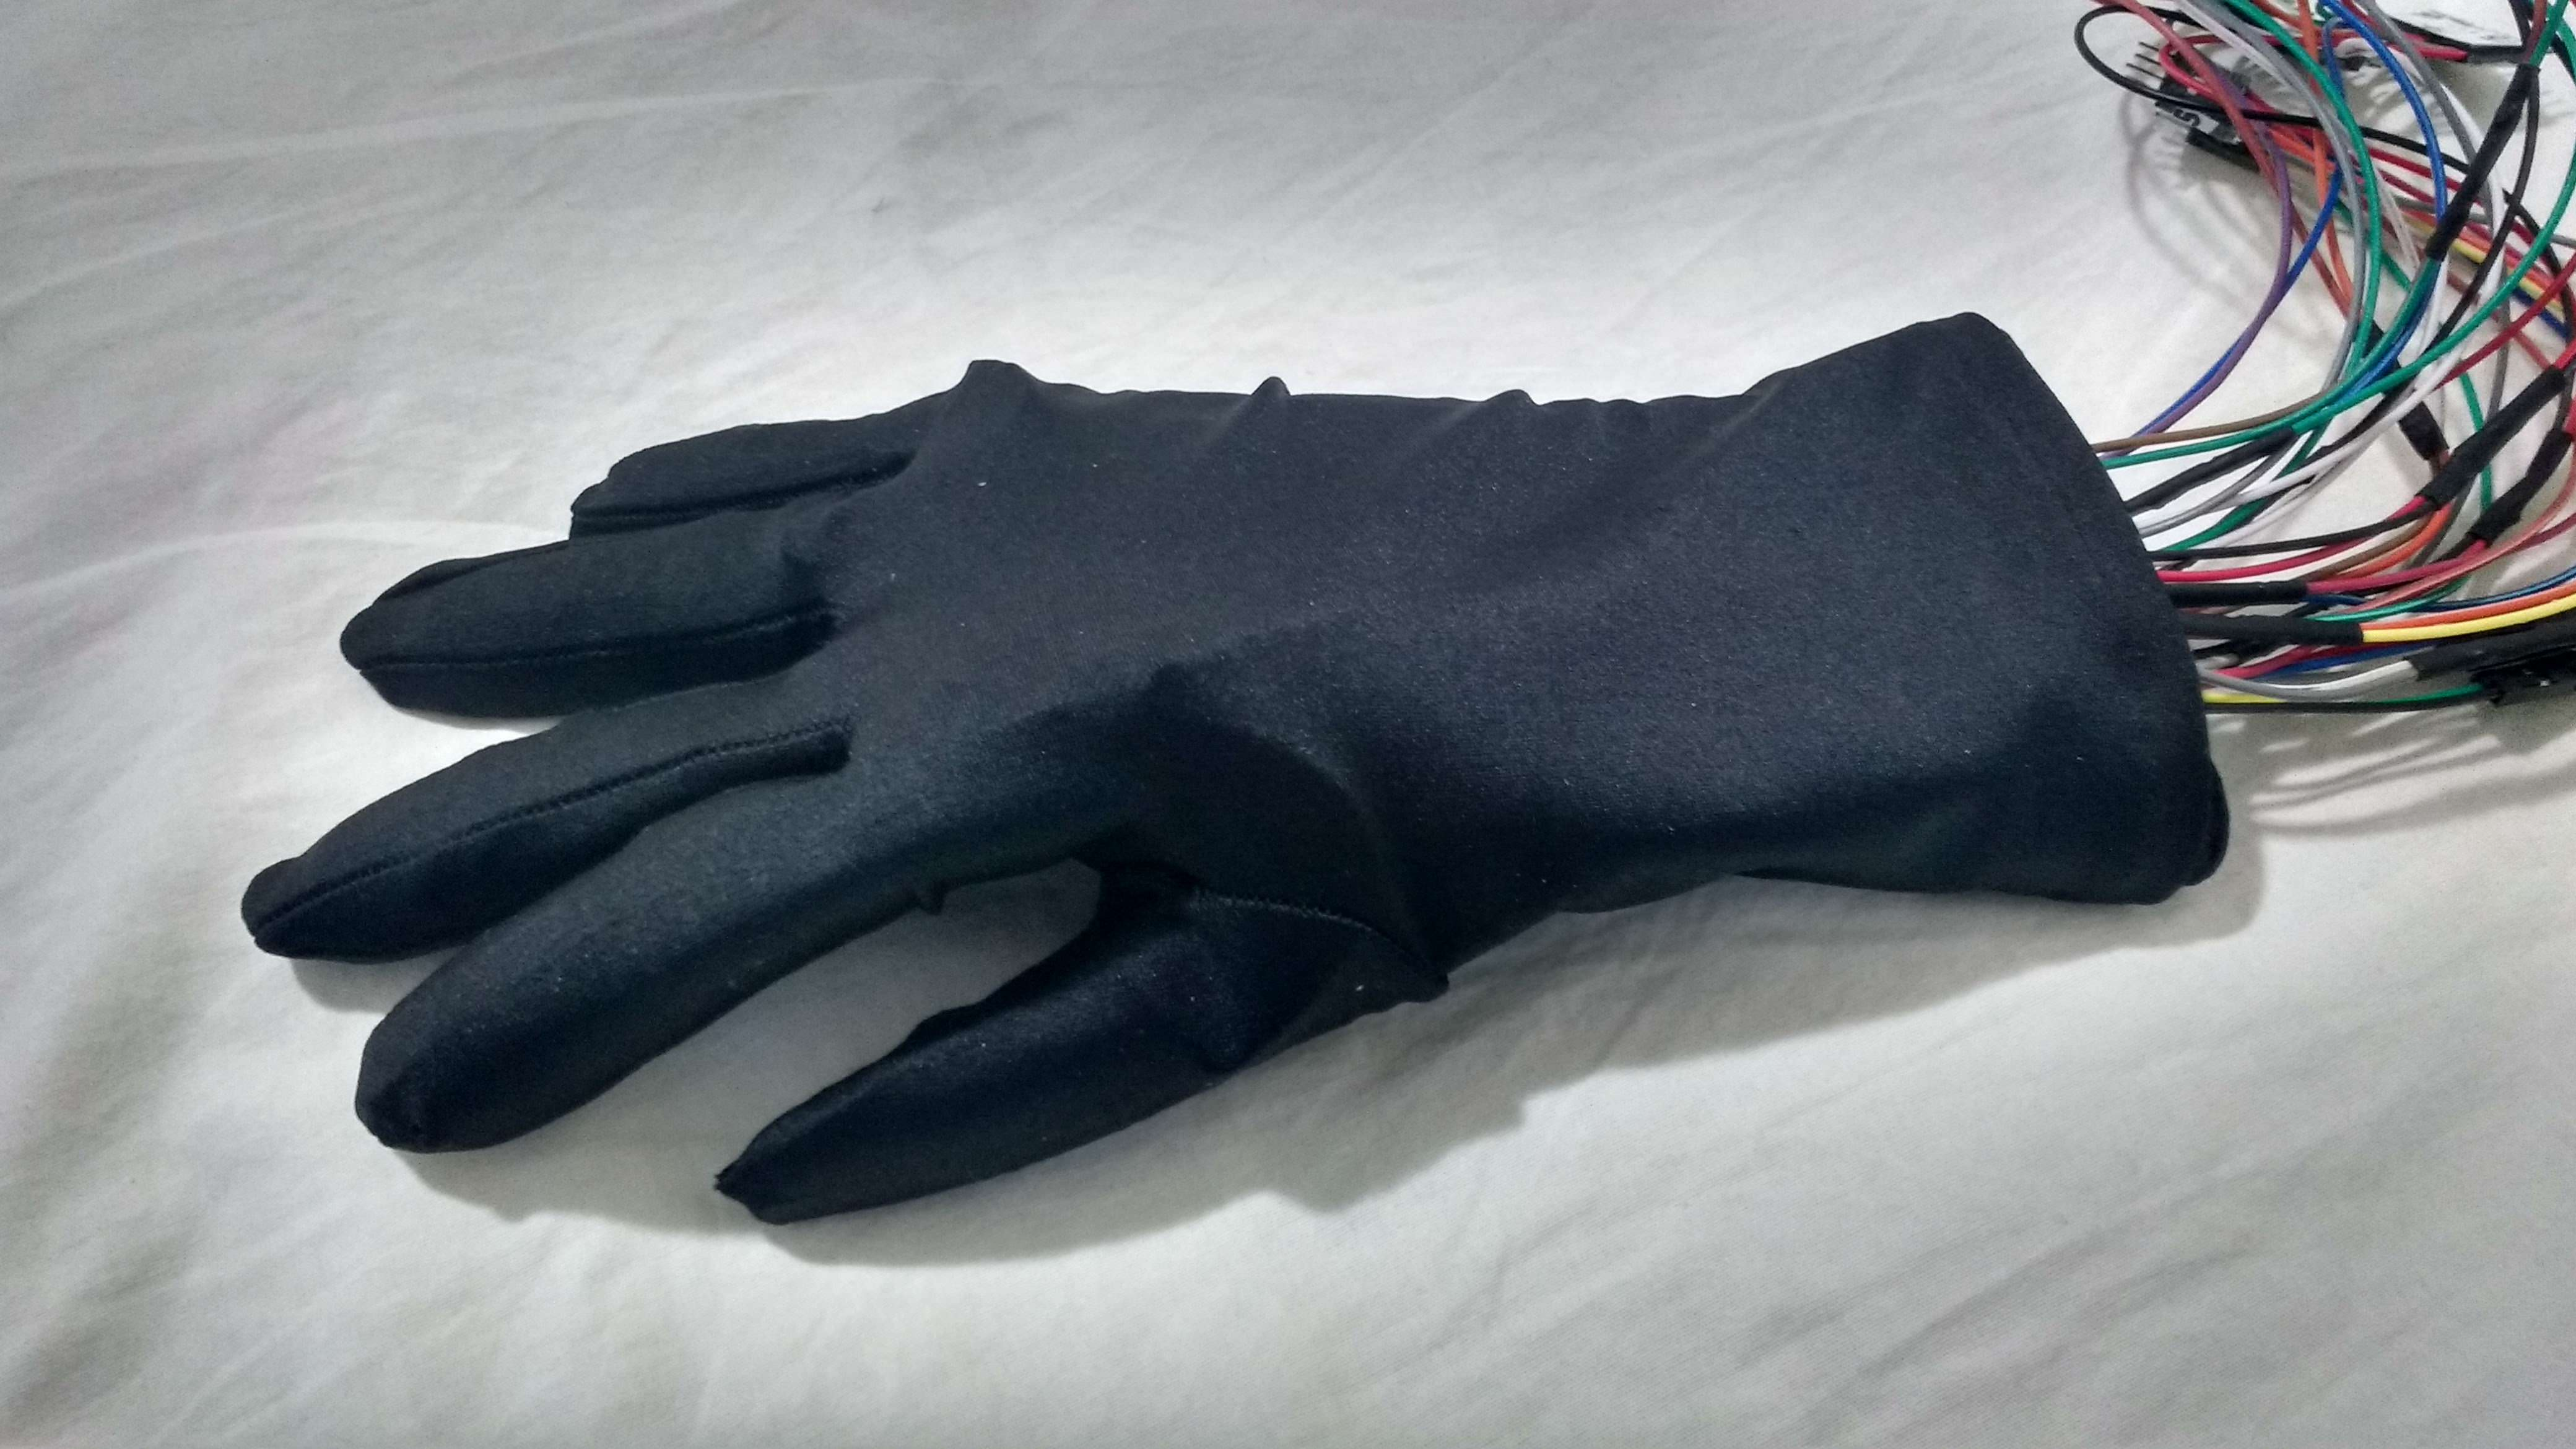
\includegraphics[width=.6\textwidth,angle =90]{imagem/luvacomlycra_mini}\label{fig:luva_lycra}}\\
  \captionsetup{justification=centering}
  \captionfont{\small{\textbf{\\Fonte: Elaborado pelo Autor}}}
  \label{fig:sensores_luva}
\end{figure}

% subsubsection sensores_de_flexão (end)

\subsection{MPU-9250} % (fold)
\label{sub:mpu_9250}
Foram utilizadas duas \ac{IMU}s \textit{MPU-9250} para conseguir obter a orientação espacial da mão. Uma \ac{IMU} foi colocada sobre as costas da mão, e a outra foi fixada no \textit{shield} de prototipagem do \textit{Arduino} que fica sobre o antebraço do usuário (Figura \ref{fig:luva_mao}). Com as \ac{IMU}s nessas posições, é possível obter os movimentos de extensão, flexão, desvio radial e ulnar do pulso. A \ac{IMU} sobre as costas da mão detecta a inclinação e rotação da mão, e a \ac{IMU} do antebraço serve como referência para o cálculo dos ângulos de dobra do pulso sobre os eixos $X$ ou $Z$ (Figura \ref{fig:maounity}).

\begin{figure}[H]
  \setlength{\abovecaptionskip}{0pt}
  \setlength{\belowcaptionskip}{0pt}
  \caption[Luva em utilização]{Luva em utilização}
  \centering
  \subfloat[Vista superior]{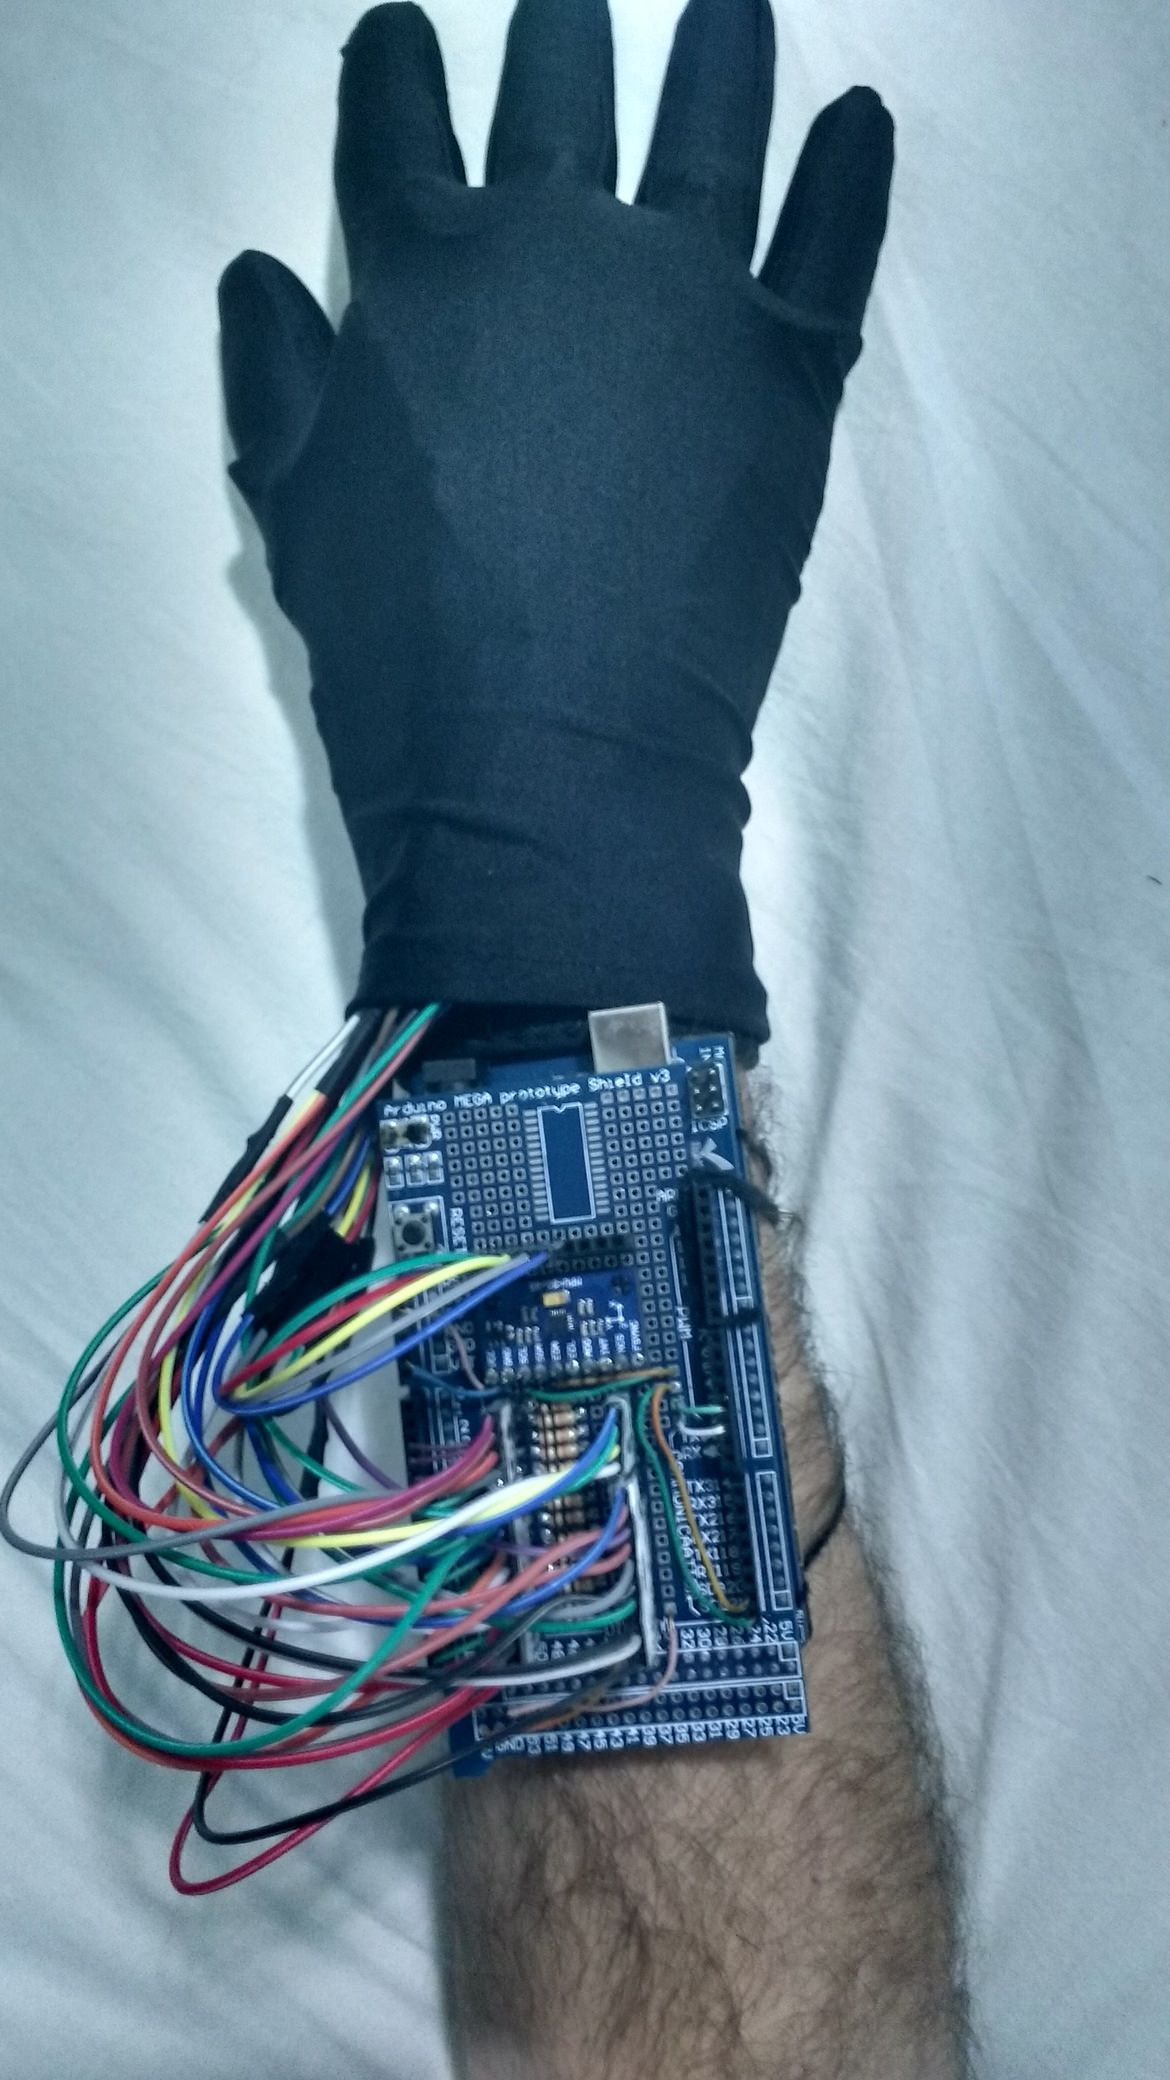
\includegraphics[width=.4\textwidth,angle=90]{imagem/luvanamaocima.jpg}\label{fig:luva_mao_cima}}]
  \\
  \subfloat[Vista lateral]{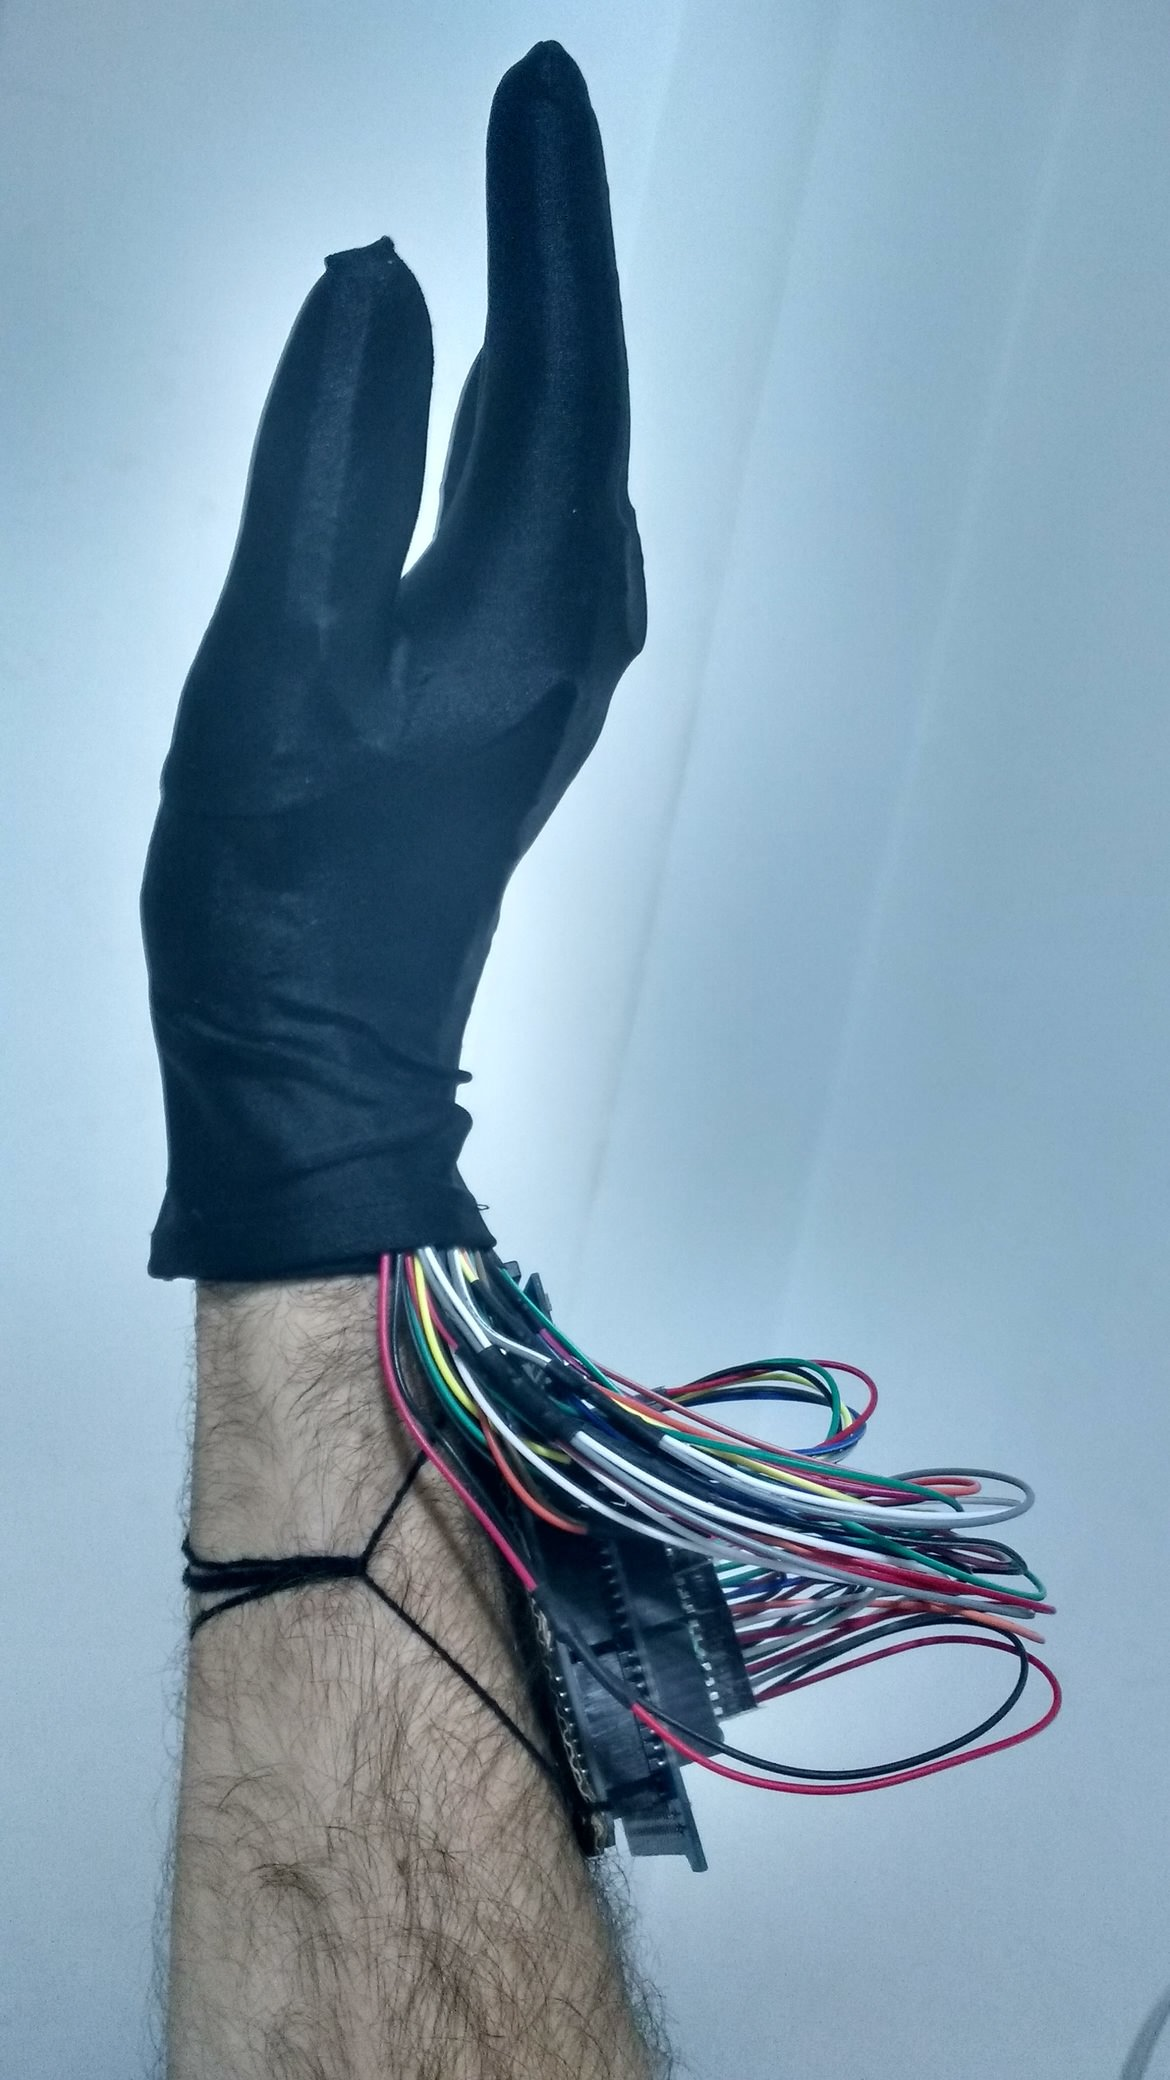
\includegraphics[width=.4\textwidth,angle =90]{imagem/luvanamaolateral.jpg}\label{fig:luva_mao_lateral}}\\
  \captionsetup{justification=centering}
  \captionfont{\small{\textbf{\\Fonte: Elaborado pelo Autor}}}
  \label{fig:luva_mao}
\end{figure}

% subsubsection mpu_9250 (end)

\subsection{Circuito} % (fold)
\label{sub:met_circuito}
O circuito elétrico (Apêndice \ref{apend:circ}) consiste nos 14 sensores de flexão, 14 resistores de \SI{10}{\kilo\ohm} e duas \ac{IMU}s \textit{MPU-9250}. Os 14 resistores e uma das \ac{IMU}s foram soldados em um \textit{shield} de prototipagem, junto com conectores para os sensores de flexão e a segunda \ac{IMU}. O circuito montado é apresentado nas Figuras \ref{fig:placacima} e \ref{fig:placabaixo}, e o circuito modificado de \citeonline{roversi} nas Figuras \ref{fig:placagusbaixo} e \ref{fig:placagusbaixo}.

Os sensores de flexão precisam dos resistores de valor fixo para que seja formado um divisor de tensão, tornando possível medir a queda de tensão no sensor, que é então detectada pelo \textit{Arduino}. Valores entre \SI{10}{\kilo\ohm} e \SI{100}{\kilo\ohm} são comuns para este tipo de sensor \cite{sparkflex} e, como os resistores de \SI{10}{\kilo\ohm} ofereceram resultados aceitáveis, esse valor foi escolhido.

As duas \ac{IMU}s são alimentadas com \SI{3.3}{\volt} e se conectam com o \textit{Arduino} através do protocolo \ac{I2C}, portanto seus pinos \ac{SCL} e \ac{SDA} se conectam aos pinos correspondentes no \textit{Arduino}. Os pinos AD0 são usados para definir o último \textit{bit} do endereço \ac{I2C} de 7 bits \cite{specmpu9250}, possibilitando que sejam conectadas duas \ac{IMU}s com endereços 0x68 (0b1101000), quando AD0 está conectado a \ac{GND} e 0x69 (0b1101001), quando conectado a \SI{3.3}{\volt}. Os pinos \ac{INT} são conectados aos pinos digitais 2 e 3, que são os pinos que podem ser utilizados para interrupções do processador do \textit{Arduino}.

Conectores de barra soldados ao \textit{shield} foram utilizados para que se possa desconectar a luva do \textit{Arduino} para facilitar o manuseio e também para permitir a realização de testes com o protótipo original.

\begin{figure}[ht!]
  \setlength{\abovecaptionskip}{0pt}
  \setlength{\belowcaptionskip}{0pt}
  \caption[Circuito no \textit{shield} de prototipagem]{Circuito no \textit{shield} de prototipagem}
  \centering
  \subfloat[Vista Superior]{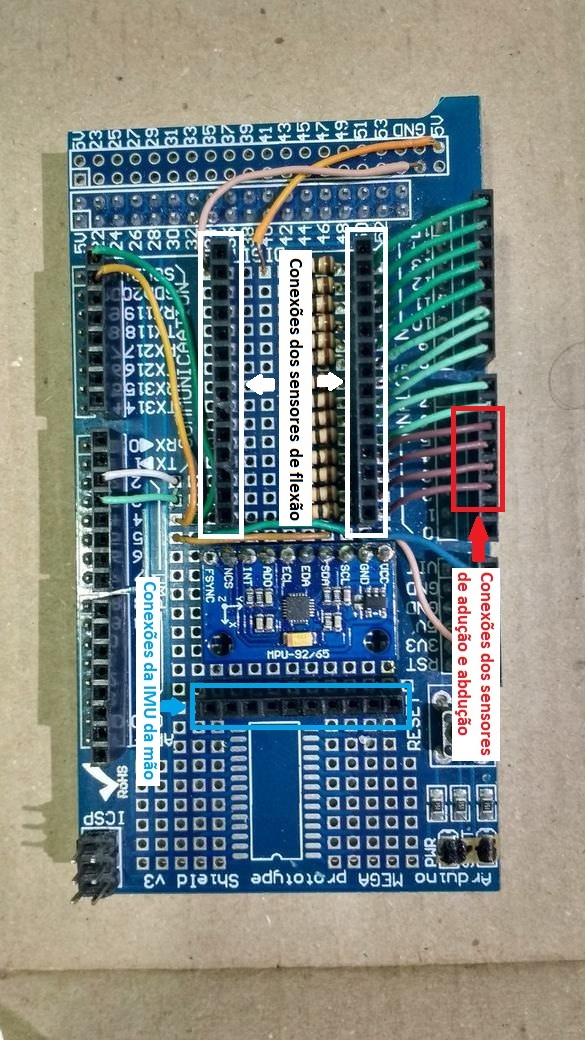
\includegraphics[trim=50 130 60 75,clip,width=.27\textwidth,angle=90]{imagem/placaCima}\label{fig:placacima}}
  \quad
  \subfloat[Vista Inferior]{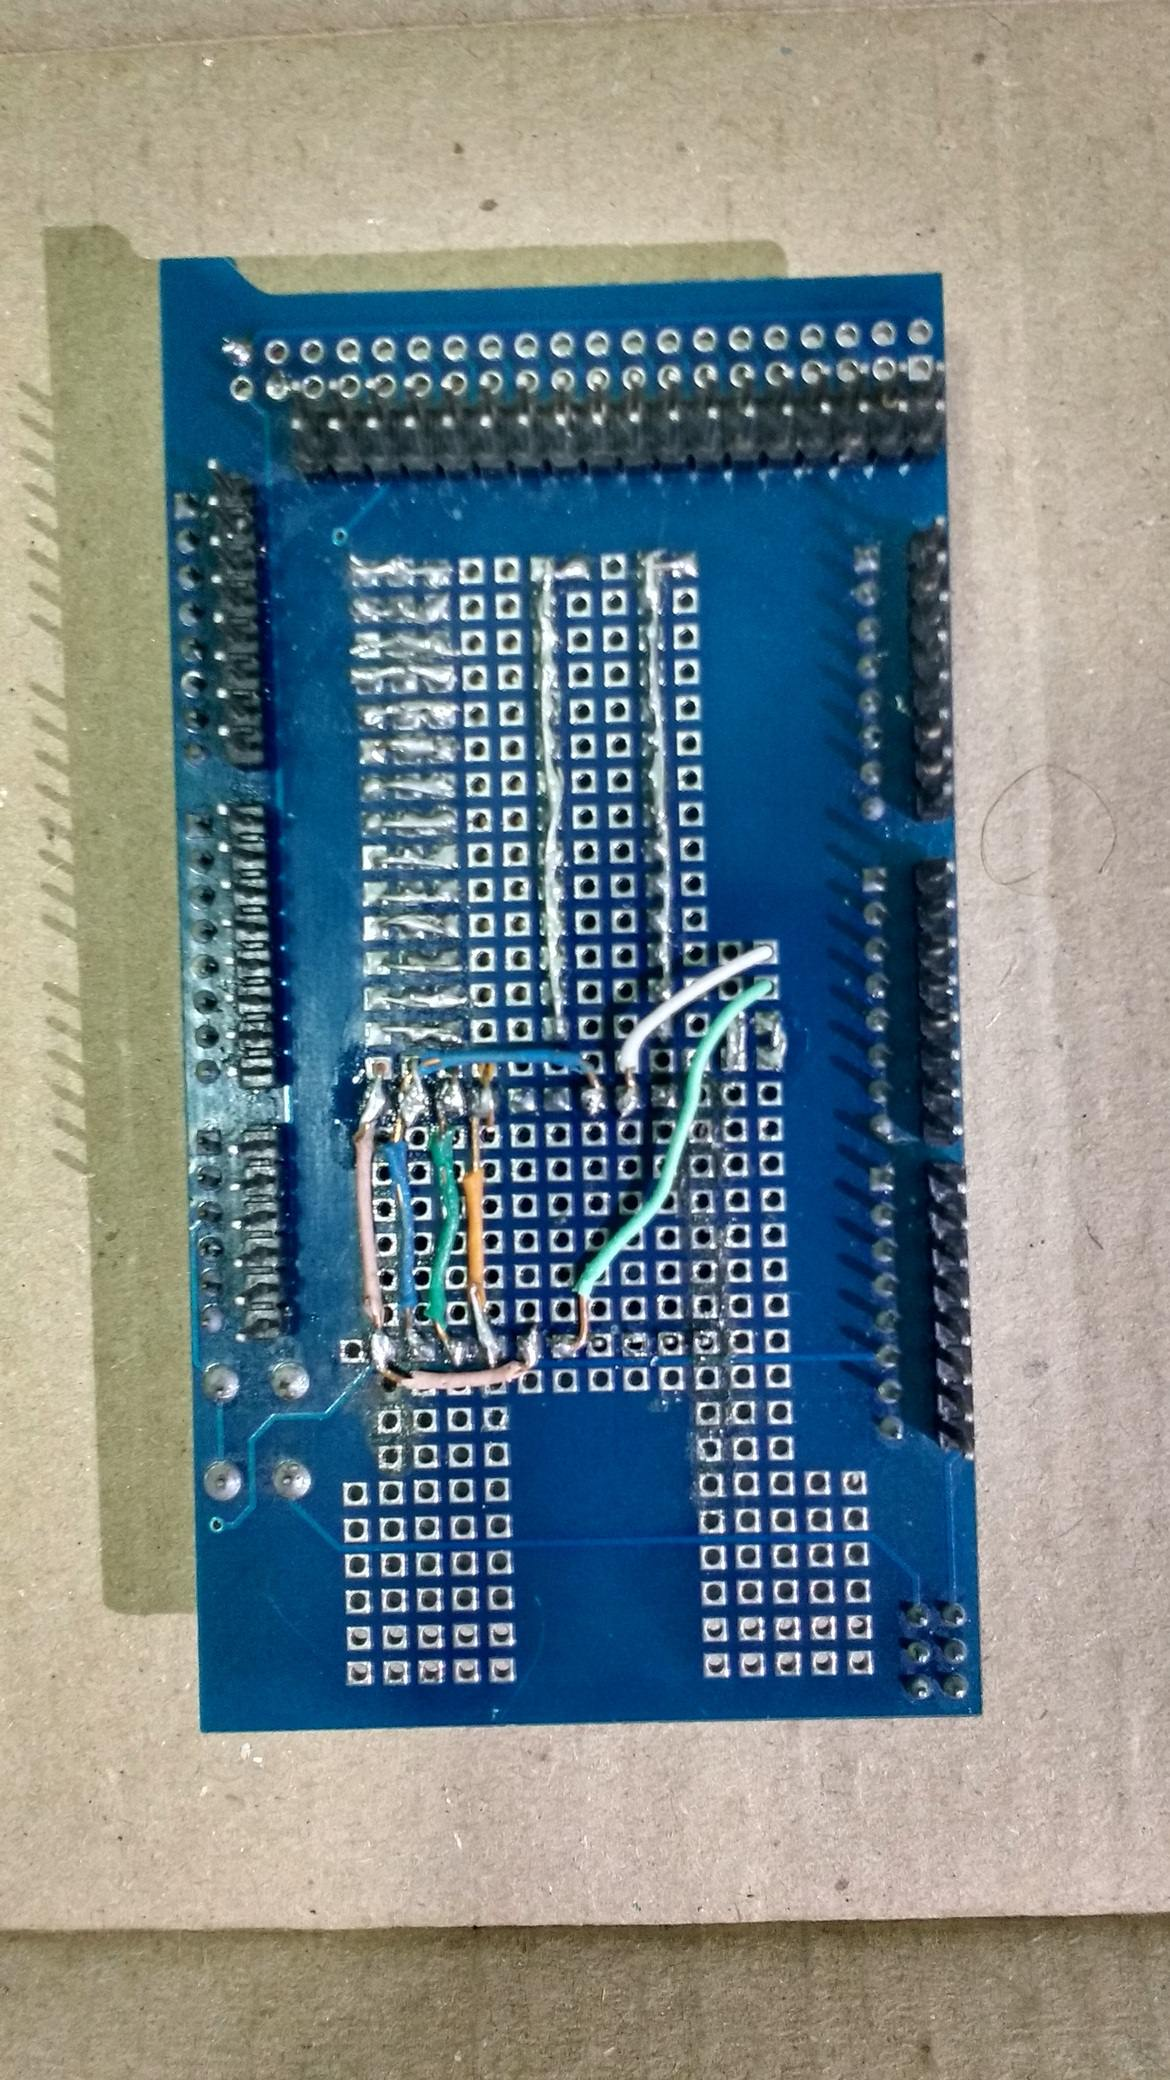
\includegraphics[trim=130 300 150 200,clip,width=.27\textwidth,angle=90]{imagem/placaBaixo}\label{fig:placabaixo}}\\
  \subfloat[Vista Superior (\citeonline{roversi})]{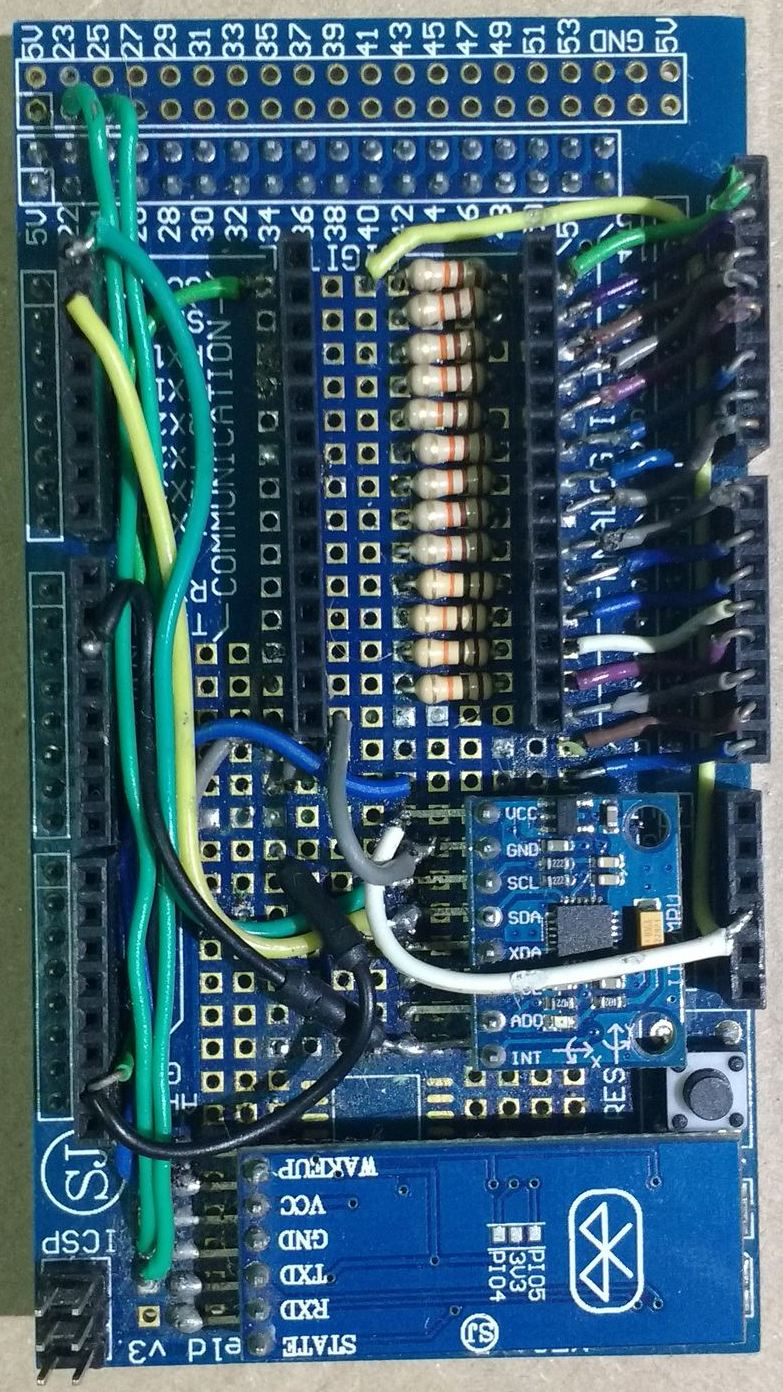
\includegraphics[width=.27\textwidth,angle=90]{imagem/placaGusCima}\label{fig:placaguscima}}
  \quad
  \subfloat[Vista Inferior (\citeonline{roversi})]{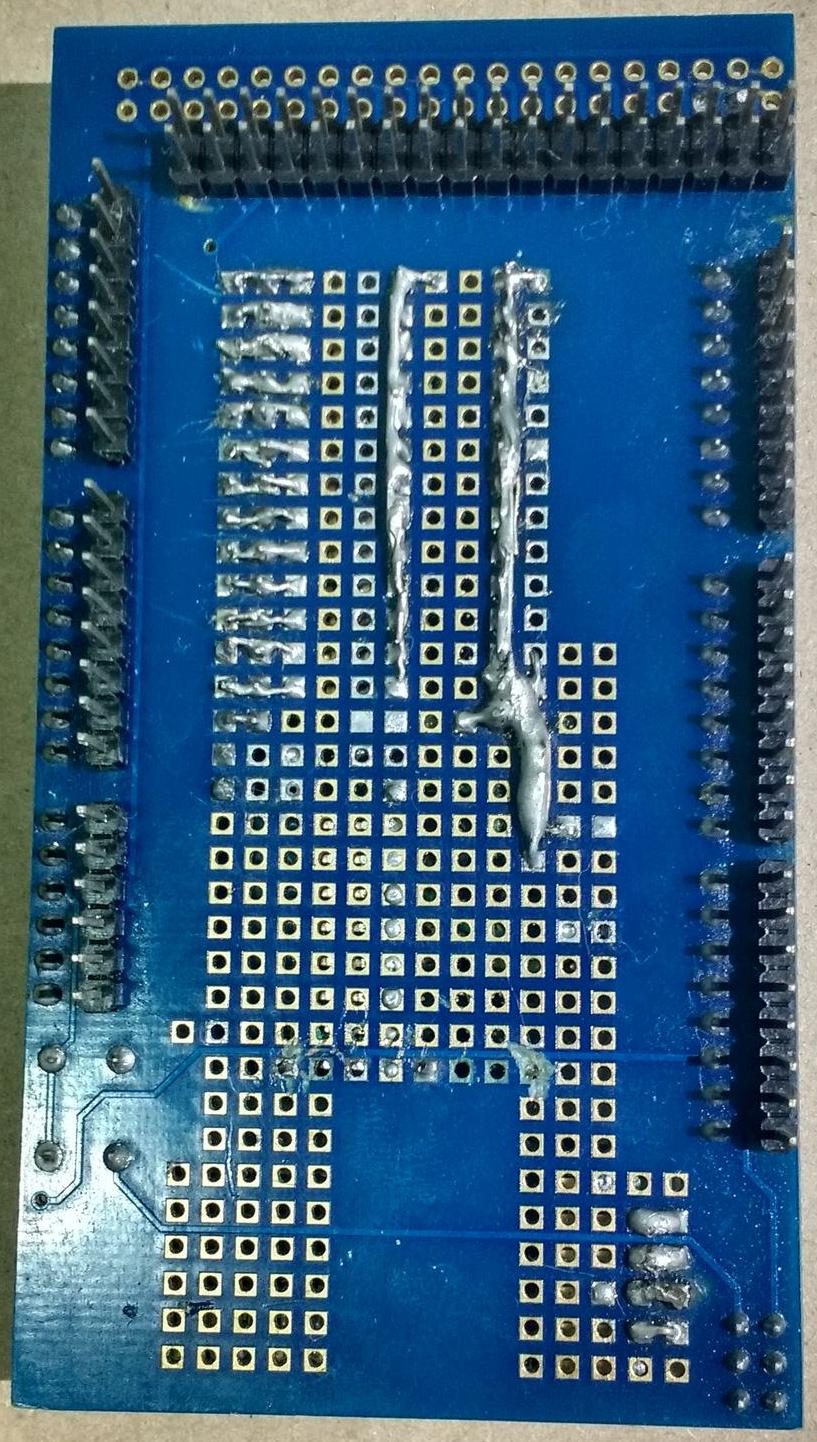
\includegraphics[width=.27\textwidth,angle=90]{imagem/placaGusBaixo}\label{fig:placagusbaixo}}
  \captionsetup{justification=centering}
  \captionfont{\small{\textbf{\\Fonte: Elaborado pelo Autor}}}
  \label{fig:shield}
\end{figure}

No novo circuito foram adicionadas as conexões para os sensores de adução e abdução e conectores de barra para todos os sensores de flexão e para a segunda \ac{IMU} que fica na mão. A \ac{IMU} que fica no \textit{Arduino} também foi rotacionada em relação à de \citeonline{roversi} para que ela tenha a mesma orientção da \ac{IMU} da mão.

% subsubsection circuito (end)
% subsection hardware (end)

\section{Software} % (fold)
\label{sec:met_software}
Nesta etapa foram implementados os códigos do \textit{Arduino} (Apêndice \ref{apend:codigoArd}) e \textit{Unity} (Apêndice \ref{apend:codigoUni}). Na Figura \ref{fig:proc} é mostrado o diagrama de processos, que mostra o funcionamento do sistema como um todo.

O \textit{Arduino} inicializa as duas \ac{IMU}s e seus respectivos \ac{DMP}s. Quando inicializados, os dados dos sensores de flexão são atualizados até que ocorra uma interrupção por parte da \textit{MPU-9250}. Quando isso ocorre, os valores de orientação são atualizados e enviados à \textit{Unity}, se essa requisitou os valores mais atuais.

A \textit{Unity} começa sua execução abrindo uma conexão com a porta serial para recebimento dos dados do \textit{Arduino}. A cada atualização de \textit{frame} é enviado um caractere pela porta serial indicando que a \textit{Unity} precisa dos dados mais recentes para atualizar as posições dos objetos. Após receber e dividir a \textit{string} contendo os dados, a posição de cada objeto é atualizada. 

\begin{figure}[H]
  \setlength{\abovecaptionskip}{0pt}
  \setlength{\belowcaptionskip}{0pt}
  \caption[Diagrama de processos]{Diagrama de processos}
  \centering
  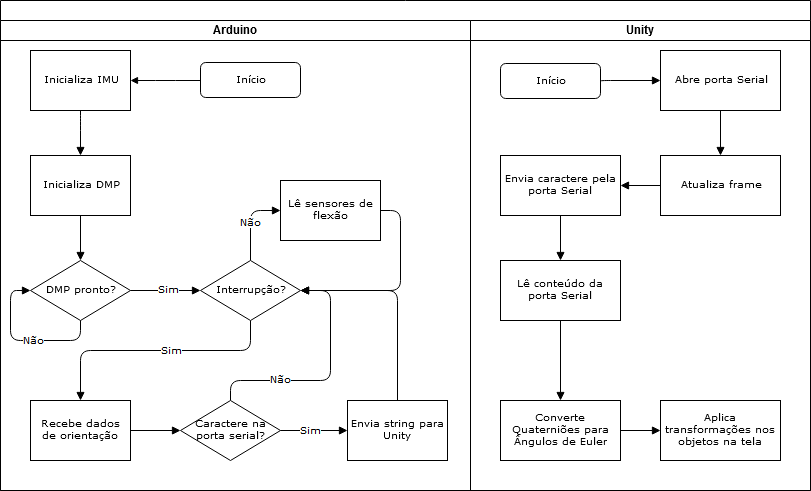
\includegraphics[width=\textwidth]{imagem/processos}
  \captionsetup{justification=centering}
  \captionfont{\small{\textbf{\\Fonte: Elaborado pelo Autor}}}
  \label{fig:proc}
\end{figure}

\subsection{Código do Arduino} % (fold)
\label{sub:codigo_do_arduino}
O código do \textit{Arduino} é responsável por ler os valores dos sensores de flexão e das \ac{IMU}s e enviá-los pela porta serial à \textit{Unity}.

Para a aquisição dos dados das \ac{IMU}s, foi utilizada a biblioteca \textit{I2Cdevlib}, de \citeonline{i2c}, que facilita a comunicação através do protocolo \ac{I2C}, que é o protocolo utilizado pelas \ac{IMU}s, e a biblioteca de \citeonline{9250DMP}, que permite a utilização e configuração do \ac{DMP} do \textit{MPU-9250}.
Para a leitura dos valores dos sensores de flexão foi utilizada a biblioteca \textit{ResponsiveAnalogRead} de \citeonline{analogread}, que reduz os ruídos das entradas analógicas do \textit{Arduino} com redução mínima de responsividade do sinal.

Como foram utilizadas duas \textit{MPU-9250}, foi preciso criar dois objetos do tipo \lstinline!MPU9250! e inicializá-los com seus respectivos endereços do \textit{bus I2C}. Também foram criados objetos do tipo \lstinline!ResponsiveAnalogRead! para cada sensor e flexibilidade passando como parâmetros o pino onde o sensor está conectado e um valor lógico indicando se o modo \textit{sleep} será ligado ou não. Quando ligado, este modo faz com que os valores lidos parem de mudar quando as variações de entrada são muito pequenas, fazendo com que haja uma pequena perda de precisão ao custo de mais responsividade. Optou-se por desligar esse modo para que se possa captar os pequenos movimentos dos dedos. O Código \ref{lst:inicMPU} mostra a inicialização dos objetos necessários.

\begin{lstlisting}[language=C++,label=lst:inicMPU,caption={Inicialização dos objetos},morekeywords={ResponsiveAnalogRead,MPU9250}]
//Inicialização das MPUs
MPU9250 mpu(0x68);
MPU9250 mpu2(0x69);

//Inicialização dos sensores
ResponsiveAnalogRead sensorPolegar1(15, false);
...
ResponsiveAnalogRead sensorAbPolInd(5, false);
ResponsiveAnalogRead sensorAbIndMed(4, false);
ResponsiveAnalogRead sensorAbMedAne(3, false);
ResponsiveAnalogRead sensorAbAneMin(2, false);
\end{lstlisting}

Também foram declaradas as variáveis globais necessárias para monitoramento das \ac{IMU}s, para os cálculos dos ângulos dos sensores e para envio da \textit{string} pela porta serial.

Na função \lstinline!setup()! do \textit{Arduino}, mostrada no Código \ref{lst:setup}, a comunicação serial foi inicializada com \textit{baud rate} de 115200. Em seguida, as \ac{IMU}s e seus \ac{DMP}s são inicializados. Se não hover falhas na inicialização, os \ac{DMP}s são ligados e os pinos de interrupção são habilitados.

\begin{lstlisting}[language=C++,label=lst:setup,caption={Função setup()},morekeywords={ResponsiveAnalogRead,MPU9250,delay,Serial,begin,println,print,attachInterrupt,pinMode}]
void setup() {
  // inicializa comunicação serial
  Serial.begin(115200);

  // inicializa dispositivos
  mpu.initialize();
  delay(100);
  mpu2.initialize();
  pinMode(INTERRUPT_PIN, INPUT);
  pinMode(INTERRUPT_PIN2, INPUT);

  // carregar e configurar o DMP
  devStatus = mpu.dmpInitialize(0x68);
  devStatus2 = mpu2.dmpInitialize(0x69);

  // Testa se inicialização ocorreu sem erros
  if (devStatus == 0 && devStatus2 == 0) {
    // liga o DMP
    mpu.setDMPEnabled(true);
    mpu2.setDMPEnabled(true);

    // Habilita detecção de interrupções do Arduino
    attachInterrupt(digitalPinToInterrupt(INTERRUPT_PIN), dmpDataReady, RISING);
    mpuIntStatus = mpu.getIntStatus();
    attachInterrupt(digitalPinToInterrupt(INTERRUPT_PIN2), dmpDataReady2, RISING);
    mpuIntStatus2 = mpu2.getIntStatus();

    // configura o flag do DMP para o Loop Principal saber se pode utilizá-lo
    dmpReady = true;
    dmpReady2 = true;

    //recebe tamanho esperado do pacote do DMP para comparação
    packetSize = mpu.dmpGetFIFOPacketSize();
    packetSize2 = mpu2.dmpGetFIFOPacketSize();
  } else {
    // ERRO - devStatus != 0
    // 1 = carregamento inicial de memória falhou
    // 2 = autalizações de connfiguração do DMP falharam
    Serial.println(F("Inicialização do DMP falhou!"));
  }
}
\end{lstlisting}

Na função \lstinline!loop()!, caso os \ac{DMP}s não tenham sido inicializados corretamente, o programa entra em \textit{loop} infinito, pois houve algum erro interno das \ac{IMU}s. Caso contrário, os valores dos sensores de flexão são atualizados (com o método \lstinline!ResponsiveAnalogRead.update()!) enquanto não há interrupções e não há \textit{bytes} para serem lidos nas filas \ac{FIFO} das \ac{IMU}s. Os valores dos sensores de flexão variam de 0 a 1024 de acordo com o quanto foram dobrados,portanto, para obter o ângulo da dobra, utilizou-se a função \lstinline!map(int value, int fromLow, int fromHigh, int toLow, int toHigh)!, que analisa o valor de entrada \lstinline!value! e retorna a conversão dos valores do intervalo \lstinline!fromLow! -- \lstinline!fomHigh! para o intervalo \lstinline!toLow! -- \lstinline!toHigh!. Para cada sensor foi obtido o valor médio das leituras com os dedos estendidos e com os dedos flexionados ao máximo para estabelecer os parâmetros \lstinline!fromLow! e \lstinline!fomHigh!, respectivamente. O parâmetro \lstinline!toLow! foi definido como 0, quando os dedos não estão dobrados, e o parâmetro \lstinline!toHigh! foi definido como \ang{90} para a flexão das articulações \ac{MCF}, \ac{IF} e \ac{IFP}, \ang{45} para a abdução da articulação \ac{MCF} do polegar e \ang{15} para a abdução das articulações \ac{MCF} dos outros dedos. Também foi utilizada a função \lstinline!constrain(val, min, max)!, que limita os possíveis valores da variável \lstinline!val! entre os valores \lstinline!min! e \lstinline!max!, para que os eventuais picos de leitura dos sensores não façam com que o modelo \ac{3D} realize movimentos naturalmente impossíveis. O Código \ref{lst:recebe_sensor_flex} mostra a aquisição dos dados dos sensores de flexão.

\begin{lstlisting}[language=C++,label=lst:recebe_sensor_flex,caption={Leitura dos sensores de flexão},morekeywords={ResponsiveAnalogRead,MPU9250,delay,Serial,begin,println,print,attachInterrupt,pinMode}]
// se programação do DMP falhou, não faça nada
if (!dmpReady || !dmpReady2) return;

// espera interrupção do DMP ou pacotes disponíveis
while ((!mpuInterrupt && fifoCount < packetSize) || (!mpuInterrupt2 && fifoCount2 < packetSize2)) {
    //Leitura dos valores dos sensores de flexibilidade
    sensorPolegar1.update();
    ...
    sensorAbPolInd.update();
    sensorAbIndMed.update();
    sensorAbMedAne.update();
    sensorAbAneMin.update();
    
    //conversão dos valores brutos dos sensores para ângulos
    PolegarGraus1   = map(sensorPolegar1.getValue(),   789, 860, 0, 70);
    constrain(PolegarGraus1,0, 70);
    ...
    grausAbPolInd   = map(sensorAbPolInd.getValue(),   784, 875, 0, -30);
    constrain(grausAbPolInd,0, -30);
    grausAbIndMed   = map(sensorAbIndMed.getValue(),   820, 858, 20, 0);
    constrain(grausAbIndMed,0, 20);
    grausAbMedAne   = map(sensorAbMedAne.getValue(),   875, 910, 20, 0);
    constrain(grausAbMedAne,0, 20);
    grausAbAneMin   = map(sensorAbAneMin.getValue(),   828, 890, 35, 0);
    constrain(grausAbAneMin,0, 35);
}

\end{lstlisting}

A Tabela \ref{tab:sens_val} mostra os pinos do \textit{Arduino} onde cada sensor de flexão está conectado, os valores brutos máximo e mínimo (adimensionais) recebidos dos sensores e os ângulos máximo e mínimo (em graus) que os sensores podem ser dobrados quando se utiliza a luva. Esses ângulos foram possíveis de serem obtidos, pois o tecido da luva limita certos movimentos, como a abdução do polegar, não permitindo a abertura máxima que seria possível sem a luva.

\begin{table}[H]
    \centering
    \footnotesize
    \setlength{\abovecaptionskip}{0pt}
    \setlength{\belowcaptionskip}{0pt}
    \caption[Relação dos valores mínimos e máximos dos sensores de flexão]{Relação dos valores mínimos e máximos dos sensores de flexão}
    \label{tab:sens_val}
    \begin{tabular}{l r r r r r}
      \hline\hline
      Sensor & Pino & Mínimo & Máximo & Ângulo Mínimo (\SI{}{\degree}) & Ângulo Máximo (\SI{}{\degree})\\
      \hline
      Polegar (MCF)              & 15 & 789 & 860 & 0 & 70\\
      Polegar (IF)               & 14 & 740 & 851 & 0 & 100\\
      Indicador (MCF)            & 13 & 761 & 884 & 0 & 80\\
      Indicador (IFP)            & 12 & 702 & 753 & 0 & 100\\
      Médio (MCF)                & 11 & 742 & 899 & 0 & 80\\
      Médio (IFP)                & 10 & 747 & 900 & 0 & 100\\
      Anelar (MCF)               & 9  & 740 & 849 & 0 & 80\\
      Anelar (IFP)               & 8  & 713 & 767 & 0 & 100\\
      Mínimo (MCF)               & 7  & 721 & 871 & 0 & 80\\
      Mínimo (IFP)               & 6  & 731 & 827 & 0 & 100\\
      Adução - Polegar/Indicador & 5  & 784 & 875 & 0 & 30\\
      Adução - Indicador/Médio   & 4  & 820 & 858 & 0 & 20\\
      Adução - Médio/Anelar      & 3  & 875 & 910 & 0 & 20\\
      Adução - Anelar/Mínimo     & 2  & 828 & 890 & 0 & 35\\
      \hline \hline
    \end{tabular}
    \\\vspace{1.3mm}
    \captionfont{\small{\textbf{Fontes: Elaborado pelo Autor}}}
\end{table}

Quando ocorrer alguma interrupção, são obtidos os valores filtrados das \ac{IMU}s no formato de Quatérnios, que são representações de orientação no espaço utilizando quatro coordenadas complexas $X$, $Y$, $Z$ e $W$. Esse formato foi escolhido pois fornecia dados mais confiáveis, o que não ocorria ao obter os valores de rotação no formato de Ângulos de Euler (ângulos em torno dos três eixos $X$, $Y$ e $Z$). Ao rotacionar a \textit{MPU-9250} em apenas um eixo, os outros dois sofriam influências quando se obtinha os dados no formato de ângulos de Euler, o que resultava em uma representação incorreta de orientação, mas utilizando quatérnios, o modelo \ac{3D} se comportou corretamente. No Código \ref{lst:recebe_orientacao}, o método \lstinline!MPU9250.dmpGetQuaternion()! obtém os dados das duas \ac{IMU}s.

\begin{lstlisting}[language=C++,label=lst:recebe_orientacao,caption={Leitura das \textit{IMUs}},morekeywords={ResponsiveAnalogRead,MPU9250,delay,Serial,begin,println,print,attachInterrupt,pinMode}]
// recebe os valores de orientação na forma de quatérnios
mpu.dmpGetQuaternion(&q, fifoBuffer);
mpu2.dmpGetQuaternion(&q2, fifoBuffer2);
\end{lstlisting}

Após obter os dados de todos os sensores, o \textit{buffer} de entrada é verificado para saber se a \textit{Unity} requisitou os valores dos ângulos e orientações. Em caso positivo, a \textit{string} era montada com os valores de orientação das duas \ac{IMU}s e os ângulos de dobra dos sensores, estes eram enviados pela porta serial e o processo era repetido. Essa lógica está representada no Código \ref{lst:envia_serial}.

\begin{lstlisting}[language=C++,label=lst:envia_serial,caption={Envio dos dados pela porta serial},morekeywords={ResponsiveAnalogRead,MPU9250,delay,Serial,begin,println,print,attachInterrupt,pinMode}]
if (Serial.available() > 0){
  //consome os bytes do buffer de entrada
  Serial.read();
  
  //Construção da string para ser escrita na porta serial
  valores  = String(PolegarGraus1) + ";"; //ângulo de dobra da MCF do Polegar
  ...
  valores += String(grausAbPolInd) + ";"; //ângulo de dobra entre Polegar e Indicador
  valores += String(grausAbIndMed) + ";"; //ângulo de dobra entre Indicador e Médio
  valores += String(grausAbMedAne) + ";"; //ângulo de dobra entre Médio e Anelar
  valores += String(grausAbAneMin) + ";"; //ângulo de dobra entre Anelar e Mínimo
  
  //orientação do braço
  valores += String(q.w,4) + ";";
  valores += String(q.x,4) + ";";
  valores += String(q.y,4) + ";";
  valores += String(q.z,4) + ";";
  
  //orientação da mão
  valores += String(q2.w,4) + ";";
  valores += String(q2.x,4) + ";";
  valores += String(q2.y,4) + ";";
  valores += String(q2.z,4);
  
  //envia valores  para porta serial
  Serial.println(valores);
}
\end{lstlisting}

% subsubsection código_do_arduino (end)

\subsection{Código da Unity} % (fold)
\label{sub:codigo_da_unity}

Primeiramente, como mostrado no Código \ref{lst:declaracao_unity}, são declaradas as variáveis e objetos necessários para utilização da porta serial e manipulações dos objetos na tela, além de variáveis para receber os dados do \textit{Arduino}. 

\begin{lstlisting}[language=C++,label=lst:declaracao_unity,caption={Declaração de variáveis da \textit{Unity}},morekeywords={SerialPort,IsOpen,Close,Open,Quaternion,GameObject,Vector3,Split,transform,localEulerAngles,Parse,Set,eulerAngles}]
//Declaração de variáveis
SerialPort serial = new SerialPort ("COM4", 115200);
public string ArduinoRead="";
public GameObject firstBone1, firstBone2, firstBone3, firstBone4, firstBone5;
public GameObject middleBone1, middleBone2, middleBone3, middleBone4, middleBone5;
public GameObject lastBone1, lastBone2, lastBone3, lastBone4, lastBone5;
public GameObject hand, arm;
public Vector3 rotacaoMao, rotacaoBraco, rotacaoFinal;
public string[] Output;
float w, x, y, z, w2, x2, y2, z2;
Quaternion quaternionBraco, quaternionMao, quaternionFinal;
\end{lstlisting}

Por padrão, um \textit{script} da \textit{Unity} precisa de duas funções: \lstinline!Start()! e \lstinline!Update()!. A função \lstinline!Start()! é executada uma vez quando a aplicação é aberta e, no caso desse projeto, é usada para abrir a comunicação com a porta serial especificada anteriormente através do método \lstinline!SerialPort.Open()!. A propriedade \lstinline!SerialPort.ReadTimeout! define a quantidade máxima de milissegundos que se deve esperar quando uma operação de leitura não termina. O valor de 100 foi escolhido, pois o envio dos dados pelo \textit{Arduino} não demora mais do que \SI{100}{\milli\second}. A função \lstinline!Start()! é mostrada no Código \ref{lst:unity_start}.

\begin{lstlisting}[language=C++,label=lst:unity_start,caption={Função Start()},morekeywords={SerialPort,IsOpen,Close,Open,Quaternion,GameObject,Vector3,Split,transform,localEulerAngles,Parse,Set,eulerAngles,ReadTimeout}]
//Configuração da conexão da porta
void Start (){
	serial.Open ();
	serial.ReadTimeout = 100;
}
\end{lstlisting}


A função \lstinline!Update()! é chamada a cada atualização de \textit{frame} e é utilizada para manipular os objetos na tela. Essa função verifica se a porta serial ainda está aberta e, em caso positivo, os dados são requisitados ao \textit{Arduino} enviando um caractere pela porta serial. Em seguida, a \textit{string} recebida é lida e armazenada na variável \lstinline!ArduinoRead!, como mostrado no Código \ref{lst:unity_update}.

A \textit{string} é uma série de valores separados por \lstinline!;!, portanto deve ser dividida com o método \lstinline!String.Split(char[] separator)!, onde \lstinline!separator! é o caractere delimitador que separa um elemento do outro na \textit{string}. O vetor resultante com os resultados é armazenado na variável \lstinline!Output!.

\begin{lstlisting}[language=C++,label=lst:unity_update,caption={Função Update()},morekeywords={SerialPort,IsOpen,Close,Open,Quaternion,GameObject,Vector3,Split,transform,localEulerAngles,Parse,Set,eulerAngles}]
void Update (){
	//verifica se a porta serial está aberta
	if (serial.IsOpen) {
		//envia caractere pela porta serial, indicando que estamos prontos para atualizar as posições
		serial.Write("o");
		
		//lê contaúdo da porta serial
		ArduinoRead = serial.ReadLine ();
		
		//separação dos valores da string
		Output = ArduinoRead.Split (new char[] { ';' }, StringSplitOptions.RemoveEmptyEntries);
...
\end{lstlisting}

O próximo passo é movimentar os objetos na tela com a propriedade \lstinline!GameObject.transform.localEulerAngles!, que recebe um vetor \ac{3D} do tipo \lstinline!Vector3(float x, float y, float z)!, onde \lstinline!x!, \lstinline!y! e \lstinline!z! são os ângulos de rotação em torno de cada eixo. A propriedade \lstinline!localEulerAngles! define os ângulos de inclinação de um objeto tomando como referência o seu objeto-pai, ou seja, o objeto ao qual ele está conectado.

O movimento das articulações \ac{MCF} em torno do eixo $Z$ se dá de acordo com os ângulos recebidos dos sensores \ac{MCF} e, o movimento do eixo $Y$ se dá de acordo com os sensores de abdução. Os sensores dos ângulos de abdução apenas detectam os ângulos entre os dedos, o que dificulta o processo de movimentação do modelo\ac{3D}, já que não há uma referência fixa a partir da qual esses ângulos seriam calculados. Para contornar esse problema, considerou-se que o dedo médio não se movimenta durante a abdução ou adução, como mencionado por \citeonline{li2009smartglove}, tornando possível o cálculo dos ângulos de abdução dos dedos indicador, anelar tendo o dedo médio como referência, e o ângulo de abdução do dedo mínimo sendo definido pela Equação \ref{eq:minimo}, onde $\theta_{\text{Médio/Anelar}}$ é a abdução entre os dedos médio e anelar, e $\theta_{\text{Anelar/Mínimo}}$ é a abdução entre os dedos anelar e mínimo. A adução do polegar já possui como referência fixa a articulação \ac{MCF} do dedo indicador.

\begin{equation}\label{eq:minimo}
    \theta_{\text{Mínimo}} = \theta_{\text{Médio/Anelar}}+\theta_{\text{Anelar/Mínimo}}
\end{equation}


Para a articulação \ac{MCF} do polegar, as rotações sobre os eixos $Y$ e $Z$ foram fixadas para compensar a posição do objeto no modelo da \textit{Unity}, já que o polegar está a um ângulo diferente dos outros dedos. As articulações \ac{IF} do polegar e \ac{IFP} dos demais dedos se movimentam apenas em torno do eixo $Z$, portanto apenas essa componente foi modificada, como mostra o Código \ref{lst:dedos_transform}. Para as articulações \ac{IFD} foi feito o cálculo mencionado em \citeonline{li2009smartglove}, onde o ângulo de dobra dessa articulação tem relação com a articulação \ac{IFP} de acordo com a Equação \ref{eq:ifd}.

\begin{equation}\label{eq:ifd}
    \theta_{IFD} = \frac{2}{3} \theta_{IFP}
\end{equation}

\begin{lstlisting}[language=C++,label=lst:dedos_transform,caption={Transformações dos dedos},morekeywords={SerialPort,IsOpen,Close,Open,Quaternion,GameObject,Vector3,Split,transform,localEulerAngles,Parse,Set,eulerAngles}]
//atualização das posições dos dedos
//Polegar
firstBone1.transform.localEulerAngles = new Vector3 (int.Parse (Output [10])-50, 225, 90);
middleBone1.transform.localEulerAngles = new Vector3 (0, 0, int.Parse (Output [0]));
lastBone1.transform.localEulerAngles = new Vector3 (0, 0, int.Parse (Output [1]));
//Indicador
firstBone2.transform.localEulerAngles = new Vector3 (0, -int.Parse (Output [11]), int.Parse (Output [2]));
middleBone2.transform.localEulerAngles = new Vector3 (0, 0, int.Parse (Output [3]));
lastBone2.transform.localEulerAngles = new Vector3 (0, 0, int.Parse (Output [3]) * 2 / 3);
//Médio
firstBone3.transform.localEulerAngles = new Vector3 (0, 0, int.Parse (Output [4]));
middleBone3.transform.localEulerAngles = new Vector3 (0, 0, int.Parse (Output [5]));
lastBone3.transform.localEulerAngles = new Vector3 (0, 0, int.Parse (Output [5]) * 2 / 3);
//Anelar
firstBone4.transform.localEulerAngles = new Vector3 (0, int.Parse (Output [12]), int.Parse (Output [6]));
middleBone4.transform.localEulerAngles = new Vector3 (0, 0, int.Parse (Output [7]));
lastBone4.transform.localEulerAngles = new Vector3 (0, 0, int.Parse (Output [7]) * 2 / 3);
//Mínino
firstBone5.transform.localEulerAngles = new Vector3 (0, int.Parse (Output [13])+int.Parse (Output [12])-10, int.Parse (Output [8]));
middleBone5.transform.localEulerAngles = new Vector3 (0, 0, int.Parse (Output [9]));
lastBone5.transform.localEulerAngles = new Vector3 (0, 0, int.Parse (Output [9]) * 2 / 3);
\end{lstlisting}

Finalmente foi realizada a transformação da mão em relação ao braço, criando os objetos do tipo \lstinline!Quaternion! e os inicializando com os valores dos quatérnios recebidos do \textit{Arduino}, como mostra o Código \ref{lst:mao_transform}. Os quatérnios são então convertidos em ângulos de Euler e é realizada a subtração dos ângulos de rotação entre a mão e o braço, a fim de obter a orientação da mão em relação ao braço, o que resulta nos movimentos de extensão, flexão e desvios radial e ulnar do pulso.

\begin{lstlisting}[language=C++,label=lst:mao_transform,caption={Transformações da mão},morekeywords={SerialPort,IsOpen,Close,Open,Quaternion,GameObject,Vector3,Split,transform,localEulerAngles,Parse,Set,eulerAngles}]
//variáveis dos quatérnios da mão e do braço
w = float.Parse (Output [14]);
x = float.Parse (Output [15]);
y = float.Parse (Output [16]);
z = float.Parse (Output [17]);
w2 = float.Parse (Output [18]);
x2 = float.Parse (Output [19]);
y2 = float.Parse (Output [20]);
z2 = float.Parse (Output [21]);

//atribuição dos objetos dos quatérnios de acordo com as variáveis anteriores
quaternionBraco.Set (x, -z, y, w);
quaternionMao.Set (x2, -z2, y2, w2);

//cálculo da diferença entre os ângulos de orientação
rotacaoFinal = quaternionMao.eulerAngles-quaternionBraco.eulerAngles;

//permite rotação do braço apenas em torno do eixo X
quaternionBraco.Set (x, 0, 0, w);

//Atualiza as rotações do braço e da mão
arm.transform.rotation = quaternionBraco;
hand.transform.localEulerAngles = rotacaoFinal;
\end{lstlisting}
% subsection código_da_unity (end)

% subsection software (end)